%!TEX root = labo.tex

\chapter{Single-Segment IP Networks}

What you will learn in this lab:
\begin{itemize}
	\item How to capture and filter network traffic
	\item How to configure a network interface for IP networking
	\item How to access IP statistics and settings with the netstat command
	\item How ARP works
	\item How hackers snoop passwords from the network
\end{itemize}

\newpage
\setsession{prelab2}
\section{Prelab 2}\label{sec:prelab2}
%!TEX root = labo.tex

\subsubsection*{New commands}
Read the manual pages of the following commands at \url{http://manpages.ubuntu.com/} for the operating system version ``\osversion'':
\begin{itemize}
	\item arp
	\item ifconfig
	\item netstat
	\item tcpdump
\end{itemize}

\subsubsection*{IP Addresses}
Read the article ``Understanding IP Addressing: Everything You Ever Wanted To Know'' by Chuck Semeria, at \url{http://holdenweb.com/static/docs/3comip.pdf}

\subsubsection*{Wireshark capture and display filters}
Go to the Wireshark website and read about capture filters and display filters for Wireshark:
\begin{itemize} 
	\item \url{http://wiki.wireshark.org/CaptureFilters}
	\item \url{http://www.wireshark.org/docs/wsug_html_chunked/ChWorkBuildDisplayFilterSection.html}.
\end{itemize}

\newpage
\subsection*{Prelab Questions}

\begin{questions}
	\q{1}{Write the syntax for an \cmd{ifconfig} command that sets the IP address of the interface \iface{eth0} to 128.143.2.3/16 with broadcast address 128.143.255.255.}
	\q{2}{Write the syntax of a \cmd{tcpdump} command that captures packets containing IP datagrams with source or destination IP address equal to 10.0.1.12.}
	\q{3}{Write the syntax of a \cmd{tcpdump} command that captures packets containing ICMP messages with source or destination IP address equal to 10.0.1.12.}
	\q{4}{Write the syntax of a \cmd{tcpdump} command that captures packets containing IP datagrams between two hosts with IP addresses 10.0.1.11 and 10.0.1.12, both on interface \iface{eth1}.}
	\q{5}{Write a \cmd{tcpdump} filter expression that captures packets containing TCP segments with source or destination IP address equal to 10.0.1.12.}
	\q{6}{Write a \cmd{tcpdump} filter expression that, in addition to the constraints in Question 5, only captures packets using port number 23.}
	\q{7}{Write the syntax for a \cmd{wireshark} command with capture filter so that all IP datagrams with source or destination IP address equal to 10.0.1.12 are recorded.}
	\q{8}{Write the syntax for a Wireshark display filter that shows IP datagrams with destination IP address equal to 10.0.1.50 and frame sizes greater than 400 bytes.}
	\q{9}{Write the syntax for a Wireshark display filter that shows packets containing ICMP messages with source or destination IP address equal to 10.0.1.12 and frame numbers between 15 and 30.}
	\q{10}{Write the syntax for a Wireshark display filter that shows packets containing TCP segments with source or destination IP address equal to 10.0.1.12 and using port number 23.}
	\q{11}{Write a Wireshark capture filter expression for Question 10.}
\end{questions}


\newpage
\setsession{lab2}
\section{Lab 2}\label{sec:lab2}

In Lab 2 you become acquainted with IP configuration issues on a single Ethernet segment. The lab also exposes you to advanced use of \cmd{tcpdump} and Wireshark.

\begin{figure}[h!t]
	\centering
	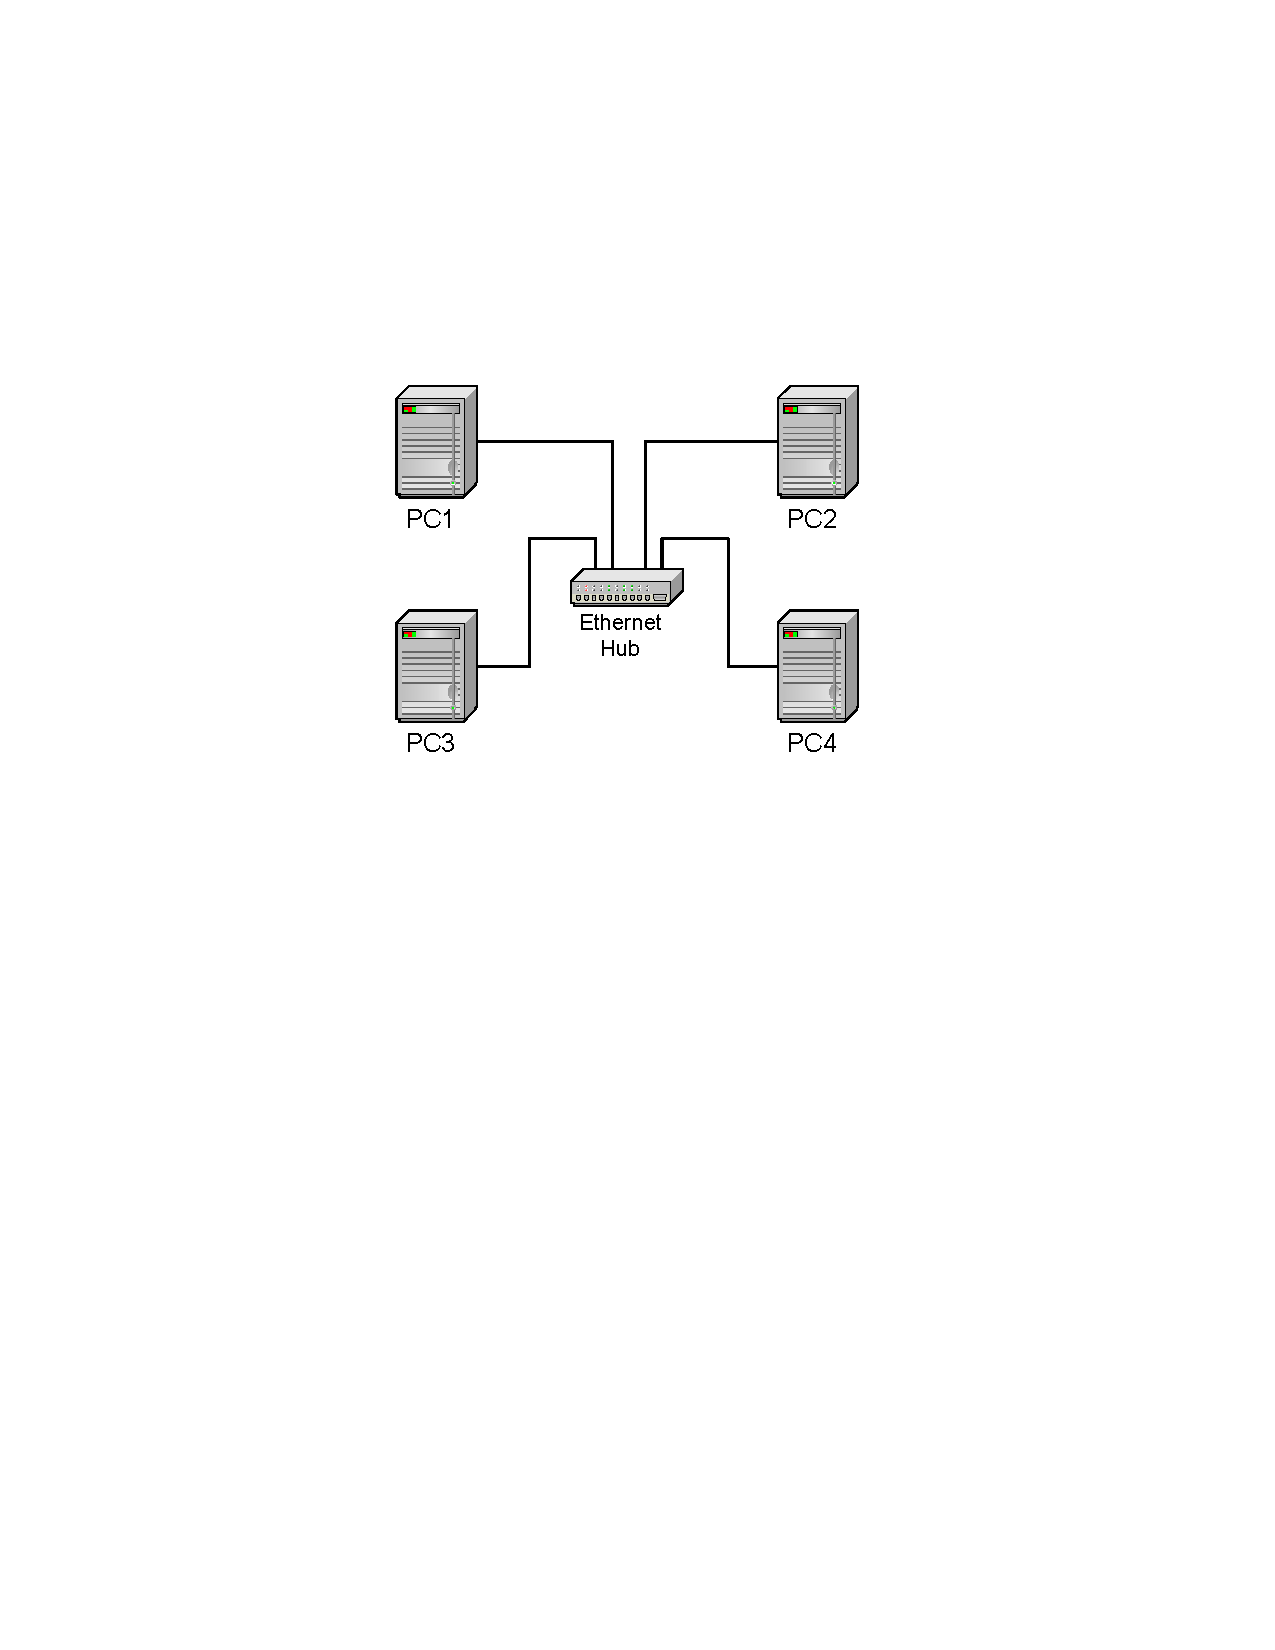
\includegraphics{graphics/lab1-network.pdf}	
	\caption{Network configuration for Lab 2.}
	\label{fig:lab2-network}
\end{figure}

The setup for this lab is identical as in Lab 1. All Linux PCs are connected to the same Ethernet segment by an Ethernet hub as shown in Figure \ref{fig:lab2-network}.
The IP addresses for the Linux PCs are configured as shown in Table \ref{tab:lab2-ip-addresses} below. Configure \iface{eth0} for each of the PCs. e.g. for PC1 use the following command.

\begin{cmdblock}
	PC1% ifconfig eth0 10.0.1.11 netmask 255.255.255.0 broadcast 10.0.255 up
\end{cmdblock}
As an alternative, you can use th \cmd{ip} command:
\begin{cmdblock}
	PC1% ip addr add 10.0.1.11/24 dev eth0
	PC1% ip link set dev eth0 up
\end{cmdblock}

\begin{table}[h!t]
	\centering
	\begin{tabular}{| c | c | c |}	
		\hline
		\textbf{Linux PC} & \textbf{IP Addresses of Ethernet Interface eth0}  \\ \hline
		PC1 & 10.0.1.11/24 \\ 
		PC2 & 10.0.1.12/24 \\
		PC3 & 10.0.1.13/24 \\
		PC3 & 10.0.1.14/24 \\ \hline
		\end{tabular}
	\caption{IPv4 addresses for Lab 2}
	\label{tab:lab2-ip-addresses}
\end{table}

\newpage
\subsection{Using filters in tcpdump}

In the first part of the lab, you explore \cmd{tcpdump} in more detail. In particular, you learn how to write filter expressions so that \cmd{tcpdump} monitors only selected traffic flows on the network. See \ref{sec:prelab2} for more details on the use of filters in \cmd{tcpdump}.

\subsubsection*{Exercise 1. Writing filter expressions for tcpdump}

In this exercise, you explore the use of simple filter expressions with the \cmd{tcpdump} command. Save the output for your lab report.

\begin{enumerate}
	\item On PC1, execute a \cmd{tcpdump} command with a filter that prints all packets with PC2 as source or destination. This command is the answer to Question 2 from the Prelab. Save the output of this \cmd{tcpdump} session to a file using the tee or tail commands discussed in Lab 1.\hspace*{\fill}
		\boxinfo{As in Lab 1, always use the \cmd{-n} option (i.e. \cmd{tcpdump -n}) to avoid that \cmd{tcpdump} tries to resolve hostnames.}
	\item In another terminal, issue a ping command to PC2 by typing \cmd{ping -c 5 10.0.1.12} on PC1 and observe the output. Recall that the ping command to a host triggers the transmission of an ICMP Echo Request. The destination host responds with an ICMP Echo Reply message.
	\item Repeat steps 1 - 2 above. In addition to the existing filter, set the filter so that only ICMP messages are captured. This command is the answer to Question 3 from the Prelab.
\end{enumerate}

\boxwarning{\textbf{Make sure to include the saved data in your lab report as they are part of your evaluation!}}

\newpage
\subsection{Using filters in Wireshark}

In this part of the lab, you experiment with filter expressions using the \cmd{wireshark} command. Recall that Wireshark has two types of filters: capture filters and display filters.

\boxinfo{There are several command line options that can be assigned when starting the \cmd{wireshark} command:\hspace*{\fill}
}
\begin{itemize}
	\item{\textbf{Capture Filters:}} A capture filter specifies the traffic to be captured by the Wireshark tool. A capture filter expression can be specified from the command line using the \cmd{-f} option or using the Wireshark GUI, under the ``Capture:Start'' menu. The syntax for specifying the filter expression is the same syntax as used by \cmd{tcpdump}.
	\item{\textbf{Display Filters:}} By default, Wireshark displays all captured packets. With a display filter, just those packets, which meet the requirements of the filter, are displayed. The display filter cannot be set from the command line. It must be entered in the ``Filter'' window at the bottom of the GUI. The syntax for setting the display filter is different from the syntax for setting a capture filter.
	\item{\textbf{Setting an interface:}} When you run Wireshark on a host with multiple network interfaces, you may specify the interface with the \cmd{-i} argument. For example, to start Wireshark to capture traffic on interface \iface{eth1}, type
		\begin{cmdblock}
	wireshark -i eth1
		\end{cmdblock}		
		If you do not specify an interface, the default is \iface{eth0}. Alternatively, you can change the interface using the Wireshark GUI, under the ``Capture:Start'' menu.
\end{itemize}

\subsubsection*{Exercise 2-A. Setting capture filters in Wireshark}
This exercise is a review of the traffic capture capabilities of Wireshark. As a new feature, you are introduced to the notion of capture filters.

\begin{enumerate}
	\item Start Wireshark on PC1 and set the same capture preferences as in Lab 1 and as shown again in Figure \ref{fig:lab2-capture-options} for your convenience. You should always set these same preferences for all your experiments.\par
		\begin{minipage}{\linewidth}
			\begin{framed}
				\centering
				\textbf{Selecting capture preferences in wireshark} \\
				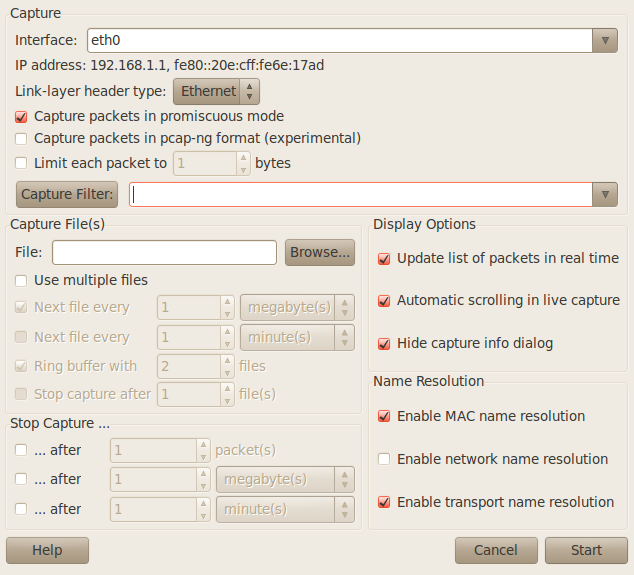
\includegraphics[width=\linewidth]{graphics/capture-options-updated.png}
				\begin{itemize}
					\item Select \iface{eth0} in ``Interface''.
					\item Select ``Capture packets in promiscuous mode''.
					\item Select ``Update list of packets in real time''.
					\item Select ``Automatic scrolling in live capture''.
					\item Unselect ``Enable MAC name resolution''.
					\item Unselect ``Enable network name resolution''.
					\item Unselect ``Enable transport name resolution''.
				\end{itemize}
			\end{framed}
			\captionof{figure}{General capture settings for Wireshark}
			\label{fig:lab2-capture-options}
		\end{minipage}
	\item Setting a capture filter: In the window ``Capture Preferences'', set a filter so that all packets that contain the IP address of PC2 are recorded. The filter is set in the ``Filter'' box under ``Capture Preferences'' (see Figure \ref{fig:lab2-capture-options}). The required filter expression is the answer to Question 7 from the Prelab.
	\item Start the capture by clicking ``OK'' in the ``Capture Preferences'' window.
	\item In another terminal window of PC1, issue a \cmd{ping} command to PC2
		\begin{cmdblock}
	PC1% ping -c 2 10.0.1.12
		\end{cmdblock}
	\item Stop the capture process of Wireshark.
	\item Save the results of the capture. This is done by selecting ``Print'' in the ``File'' menu as described in Lab 1. (As instructed in Lab 1, unless asked to save the details of captured frames, selecting the summary option is usually sufficient.)
\end{enumerate}

\boxwarning{\textbf{Make sure to include the saved data in your lab report as they are part of your evaluation!}}

\subsubsection*{Exercise 2-B. Working with display filters}

Next you set display filters, which allow you to select a subset of the captured data for display in the main window of Wireshark.

\begin{enumerate}
	\item In the Wireshark main window on PC1 from Exercise 2-A, set the display options as listed below. You can find the display options in the ``Capture Options'' window (select "Start" in the "Capture" menu)(see Figure \ref{fig:lab2-capture-options}):\par
		\begin{itemize}
			\item Select ``Update list of packets in real time''.
			\item Select ``Automatic Scrolling in live capture''.
			\item Unselect ``Enable MAC name resolution''.
			\item Unselect ``Enable network name resolution''.
			\item Unselect ``Enable transport name resolution''.
		\end{itemize}
	\item Setting a display filter: Type the desired display filter in the field next to the ``Filter'' box, which is located at the bottom of the Wireshark main window, as shown in Figure \ref{fig:lab2-display-filter}. Click the ``Reset'' button next to the ``Filter'' box to clear any existing filter:\par
		\begin{minipage}{\linewidth}
			\centering
			
\includegraphics[width=\linewidth]{graphics/display-filter-updated.png}
			\captionof{figure}{Filter box for setting display filters.}
			\label{fig:lab2-display-filter}
		\end{minipage}
		Enter a display filter so that all IP datagrams with destination IP address 10.0.1.12 are shown. Refer to Question 8 from the Prelab.
	\item Observe the changes in the display panel of Wireshark. Only packets with 10.0.1.12 in the IP destination address field are now being displayed.
	\item Save the displayed data, by selecting ``File:Print''. Note that the ``Print'' command only saves packets that are currently being displayed. If a display filter is used, the saved data is limited to the packets that match the display filter.
	\item Repeat the above exercise with a display filter that lists only IP datagrams with source IP address equal to 10.0.1.12. Save the results.		
\end{enumerate}

\boxwarning{\textbf{Make sure to include the saved data in your lab report as they are part of your evaluation!}}

\subsubsection{Exercise 2-C. More complex capture and display filters}

In this exercise, you learn how to use more sophisticated filters to restrict the packets being captured and displayed.

\begin{enumerate}
	\item Start Wireshark on PC1 and start to capture traffic using the same settings as in Exercise 2-A. Do not set any capture or display filters!
	\item From a new terminal on PC1, execute the \cmd{ping} command for PC2 
		\begin{cmdblock}
	PC1% ping -c 5 10.0.1.12
		\end{cmdblock}
	\item At the same time, start a Telnet session from PC1 to PC2 in another terminal by typing
		\begin{cmdblock}
	PC1% telnet 10.0.1.12
		\end{cmdblock}
		and log in as \textit{telecomlabo}. After you logged in successfully to PC2, logout with the command \cmd{exit}.
	\item Stop the traffic capture of wireshark.
	\item Apply a set of display filters to the captured traffic and save the output to a text file. Select the option ``Print summary'' in the ``Print'' window.
		\begin{itemize}
			\item Display packets that contain ICMP messages with the IP address of PC2 either in the IP destination address or IP source address. Refer to Question 9 from the Prelab. Save the output.
			\item Display packets that contain TCP traffic with the IP address of PC2 either in the IP destination address or IP source address. Refer to Question 10 from the Prelab. Save the output.
			\item Display packets that, in addition to the constraints in the previous filter expression, use the port number 23. Refer to Question 10 from the Prelab. Save the output.
		\end{itemize}
\end{enumerate}

\boxwarning{\textbf{Make sure to include the saved data in your lab report as they are part of your evaluation!}}

\newpage
\subsection{ARP - Address Resolution Protocol}

This part of the lab explores the operation of the Address Resolution Protocol (ARP) which resolves a MAC address for a given IP address. The lab exercises use the Linux command \cmd{arp} for displaying and manipulating the contents of the ARP cache. The ARP cache is a table that holds entries of the form \textless IP address, MAC address\textgreater.

\boxinfo{The most common uses of the \cmd{arp} command are as follows:
	\begin{description}
		\item[\texttt{arp -a}]\hfill \\
			Displays the content of the ARP cache.
		\item[\texttt{arp -d \textless IPAddress\textgreater}] \hfill \\
			Deletes the entry with IP address IPAddress.
		\item[\texttt{arp -s \textless IPAddress\textgreater \textless MAC\_Address\textgreater}] \hfill \\
			Adds a static entry to the ARP cache which is never overwritten by network events. The MAC address is entered as a 6 hexadecimal bytes separated by colons.\\
			Example: \texttt{arp -s 00:02:2D:0D:68:C1}
	\end{description}
}

\boxinfo{\textbf{Time-outs in the ARP cache:}\hfill \\
	The entries in an ARP cache have a limited lifetime. Entries are deleted unless they are refreshed. The typical lifetime of an ARP entry is 2 minutes, but much longer lifetimes (up to 20 minutes) have been observed. You may want to verify when your Linux system does remove ARP entries automatically after a certain amount of time.}

\boxinfo{\textbf{Refreshing the ARP cache:}\hfill \\
	In Linux, you will observe that occasionally, a host sends out ARP requests to interfaces that are already in the ARP cache. Example: Suppose that a host with IP address 10.0.1.12 has an ARP cache entry: ``\textless10.0.1.11\textgreater is-at \textless00:02:83:39:2C:42\textgreater''. Then, this host occasionally sends a unicast ARP Request to MAC address 00:02:83:39:2C:42 of the form ``Who has 10.0.1.11? Tell 10.0.1.12'' to verify that the IP address 10.0.1.11 is still present before deleting the entry from the ARP cache.}

\subsubsection*{Exercise 3-A. A simple experiment with ARP}
\begin{enumerate}
	\item On PC1, view the ARP cache with \cmd{arp -a} and delete all entries with the \cmd{-d}  option.
	\item Start Wireshark on PC1 with a capture filter set to the IP address of PC2.
	\item Issue a ping command from PC1 to PC2:
		\begin{cmdblock}
	PC1% ping -c 2 10.0.1.12
		\end{cmdblock}
	Observe the ARP packets in the Wireshark window. Explore the MAC addresses in the Ethernet headers of the captured packets. Direct your attention to the following fields:
		\begin{itemize}
			\item The destination MAC address of the ARP Request packets.
			\item The Type field in the Ethernet headers of ARP packets and ICMP messages.
		\end{itemize}
	\item View the ARP cache again with the command \cmd{arp -a}. Note that ARP cache entries get refreshed/ deleted fairly quickly (approx. 2 minutes).
	\item Save the results of Wireshark to a pcap dump file.
\end{enumerate}

Use the saved data to answer to the following questions:

\begin{questions}
	\q{3.A.1}{What is the destination MAC address of an ARP Request packet?}
	\q{3.A.2}{What are the different values of the Type field in the Ethernet headers that you observed?}
	\q{3.A.3}{Use the captured data to discuss the process in which ARP acquires the MAC address for IP address 10.0.1.12.}
\end{questions}
	
\subsubsection*{Exercise 3-B. Matching IP addresses and MAC addresses}
Identify the MAC addresses of all interfaces connected to the network, and enter them in Table \ref{tab:lab2-ip-to-mac}. You can obtain the MAC addresses from the ARP cache of each PC. You can fill up the ARP cache at a host, by issuing a ping command from that host to every other host on the network. Alternatively, you can obtain the MAC addresses from the output of the \cmd{ifconfig -a} command explained in Part 5.

\begin{table}[h!t]
	\centering
	\begin{tabular}{| c | c | c |}	
		\hline
		\textbf{Linux PC} & \textbf{IP Address of eth0} & \textbf{MAC Address of eth0} \\ \hline
		PC1 & 10.0.1.11/24 & \\ 
		PC2 & 10.0.1.12/24 & \\
		PC3 & 10.0.1.13/24 & \\
		PC3 & 10.0.1.14/24 & \\ \hline
	\end{tabular}
	\caption{ IP and MAC addresses.}
	\label{tab:lab2-ip-to-mac}
\end{table}

\begin{questions}
	\q{3.B.1}{Include the completed Table \ref{tab:lab2-ip-to-mac} in your lab report.}
\end{questions}

\subsubsection*{Exercise 3-C. ARP requests for a non-existing address}

Observe what happens when an ARP Request is issued for an IP address that does not exist.

\begin{enumerate}
	\item On PC1, start wireshark with a capture filter set to capture packets that contain the IP address of PC1:
		\begin{cmdblock}
	PC1% wireshark -f 'host 10.0.1.11'
		\end{cmdblock}
	\item Establish a Telnet session from PC1 to 10.0.1.10 (Note that this address does not exist on this network)
		\begin{cmdblock}
	PC1% telnet 10.0.1.10
		\end{cmdblock}
		Observe the time interval and the frequency with which PC1 transmits ARP Request packets. Repeat the experiment a number of times to discover the pattern.
	\item Save the captured output.
\end{enumerate}

\begin{questions}
	\q{3.C.1}{Using the saved output, describe the time interval between each ARP Request packet issued by PC1. Describe the method used by ARP to determine the time between retransmissions of an unsuccessful ARP Request. Include relevant data to support your answer.}
	\q{3.C.2}{Why are ARP Request packets not transmitted (i.e. not encapsulated) as IP packets? Explain your answer.}
\end{questions}

\newpage
\subsection{The netstat command}

The Linux command \cmd{netstat} displays information on the network configuration and activity of a Linux system, including network connections, routing tables, interface statistics, masquerade connections, and multicast memberships. The following exercise explores how to use the \cmd{netstat} command to extract different types of information about the network configuration of a host.

\boxinfo{The most common uses of the \cmd{netstat} command are as follows:
	\begin{description}
		\item[\texttt{netstat -i}]\hfill \\
			Displays a table with statistics of the currently configured network interfaces.
		\item[\texttt{netstat -rn}] \hfill \\
			Displays the kernel routing table. The \cmd{-n} option forces \cmd{netstat} to print the IP addresses. Without this option, \cmd{netstat} attempts to display the hostnames.
		\item[\texttt{netstat -an; netstat -tan; netstat -uan}] \hfill \\
			 Displays the active network connections. The \cmd{-a} option displays all active network connections, the \cmd{-ta} option displays only information on TCP connections, and the \cmd{-ua} option displays only information on UDP traffic. Omitting the \cmd{-n} options prints hostnames and names of servers, instead of IP addresses and ports numbers.
		\item[\texttt{netstat -s}] \hfill \\
			Displays summary statistics for each protocol that is currently running on the host.
	\end{description}
}


\subsubsection*{Exercise 4. Basic usage of the netstat command}
On PC1, try the different variations of the \cmd{netstat} command listed above and save the output to a file.

\begin{enumerate}
	\item Display information on the network interfaces by typing
		\begin{cmdblock}
	PC1% netstat -in
		\end{cmdblock}
	\item Display the content of the IP routing table by typing
		\begin{cmdblock}
	PC1% netstat -rn
		\end{cmdblock}
	\item Display information on TCP and UDP ports that are currently in use by typing
		\begin{cmdblock}
	PC1% netstat -a
		\end{cmdblock}
	\item Display the statistics of various networking protocols by typing
		\begin{cmdblock}
	PC1% netstat -s
		\end{cmdblock}
\end{enumerate}

\boxinfo{The values of the statistics displayed by some of the \cmd{netstat} commands are reset each time a host is rebooted.}


\begin{questions}
	\q{4.1}{Attach the saved output to your report. Using the saved output, answer the following questions.}
	\q{4.1.a}{What are the network interfaces of PC1 and what are the MTU (Maximum Transmission Unit) values of the interfaces?}
	\q{4.1.b}{How many IP datagrams, ICMP messages, UDP datagrams, and TCP segments has PC1 transmitted and received since it was last rebooted?}
	\q{4.2}{Explain the role of interface lo, the loopback interface. In the output of "netstat -in", why are the values of RX-OK (packets received) and TX-OK (packets transmitted) different for interface "eth0" but identical for interface lo?}
\end{questions}

\newpage	
\subsection{Configuring IP interfaces in Linux}

The \cmd{ifconfig} command is used to configure parameters of network interfaces on a Linux system, such as enabling and disabling of interfaces and setting the IP address. The \cmd{ifconfig} command is usually run when a system boots up. In this case, the parameters of the commands are read from a file. Once the Linux system is running, the \cmd{ifconfig} command can be used to modify the network configuration parameters.

\boxinfo{The most common uses of the \cmd{ifconfig} command to query the status of network interfaces are as follows:
	\begin{description}
		\item[\texttt{ifconfig}]\hfill \\
			Displays the configuration parameters of all active interfaces.
		\item[\texttt{ifconfig -a}] \hfill \\
			Displays the configuration parameters of all network interfaces, including the inactive interfaces.
		\item[\texttt{ifconfig \textless interface>\textgreater}] \hfill \\
			Displays the configuration parameters of a single interface. For example, \cmd{ifconfig eth0} displays information on interface \iface{eth0}.
	\end{description}
}

\boxinfo{There are numerous options for configuring a network interface with \cmd{ifconfig}. The following example shows how to enable and disable an interface and how to change the IP configuration.
	\begin{description}
		\item[\texttt{ifconfig eth0 down}]\hfill \\
			Disables the eth0 interface. No traffic is sent or received on a disabled interface.
		\item[\texttt{ifconfig eth0 up}]\hfill \\
			Enables the eth0 interface.
		\item[\texttt{ifconfig eth0 10.0.1.8 netmask 255.255.255.0 broadcast 10.0.1.255}]\hfill \\
			Assigns interface \iface{eth0} the IP address 10.0.1.8/24 and a broadcast address of 10.0.1.255. The interface should be disabled before a new IP address is assigned, and should be enabled after the IP address has been modified.
		\item[\texttt{ifconfig eth0 down 10.0.1.8 netmask 255.255.255.0 broadcast 10.0.1.255 up}]\hfill \\
			Performs all three commands above in sequence. Interface \iface{eth0} is disabled, an IP address and a broadcast address are assigned, and the interface is enabled.
		\item[\texttt{ifconfig eth0 mtu 500}]\hfill \\
			Sets the MTU of interface \iface{eth0} to 500 bytes.
	\end{description}
}

\subsubsection*{Exercise 5. Changing the IP address of an interface}

Use the \cmd{ifconfig} command to modify the IP address of the \iface{eth0} interface of PC4.
\begin{enumerate}
	\item On PC4, run \cmd{ifconfig -a} and save the output.
	\item Change the IP address of interface \iface{eth0} of PC4 to 10.0.1.11/24.
	\item Run \cmd{ifconfig -a} again and save the output.
\end{enumerate}

\begin{questions}
	\q{5.1}{Attach the saved files to your report and explain the fields of the \cmd{ifconfig} output.}
\end{questions}
	
\newpage
\subsection{Duplicate IP addresses}
In this part of the lab, you observe what happens when two hosts have identical IP addresses.

\subsubsection*{Exercise 6. Duplicate IP addresses}
\begin{enumerate}
	\item After completing Exercise 5, the IP addresses of the Ethernet interfaces on the four PCs are as shown in the Table \ref{tab:lab2-ip-addresses-part-6}. Note that PC1 and P4 are assigned the same IP address.

		\begin{table}[h!t]
			\centering
			\begin{tabular}{| c | c | c |}	
				\hline
				\textbf{Linux PC} & \textbf{IP Addresses of Ethernet Interface eth0}  \\ \hline
				PC1 & 10.0.1.11/24 \\ 
				PC2 & 10.0.1.12/24 \\
				PC3 & 10.0.1.13/24 \\
				PC3 & 10.0.1.11/24 \\ \hline
			\end{tabular}
			\caption{IP addresses for Part 6}
			\label{tab:lab2-ip-addresses-part-6}
		\end{table}
	\item Delete all entries in the ARP cache on all PCs.
	\item Run wireshark on PC3 and capture the network traffic to and from the duplicate IP address 10.0.1.11
	\item From PC3, start a Telnet session to the duplicate IP address, 10.0.1.11, by typing
		\begin{cmdblock}
	PC3% telnet 10.0.1.11
		\end{cmdblock}
		and log in as \textit{telecomlabo} user, using the \textit{mvkbj1n} password.
	\item Once you have logged in, determine the name of the host to which you are connected. The name of the host can be determined in several ways: (1) issue the command \cmd{hostname}, (2) inspect the ARP cache on PC3, or (3) interpret the captured Wireshark packets.
	\item Stop the traffic capture in Wireshark.
	\item Save all ARP packets and the first few TCP packets captured by Wireshark. Also save the ARP cache of PC3 using the \cmd{arp -a} command.
	\item When you are done with the exercise, reset the IP address of PC4 to its original value as given in Table \ref{tab:lab2-ip-addresses}.
\end{enumerate}

\begin{questions}
	\q{6.1}{Explain why the Telnet session was established to one of the hosts with the duplicate address and not the other. Explain why the Telnet session was established at all, and did not result in an error message. Use the ARP cache and the captured packets to support your explanation.}
\end{questions}

\newpage
\subsection{Changing netmasks}

In this part of the lab you test the effects of changing the netmask of a network configuration. In the table below, two hosts (PC2 and PC4) have been assigned different network prefixes.

\boxwarning{If you are having difficulties understanding the concept of netmasks, try using a subnet calculator tool. You can find one at  \url{http://subnet-calculator.com} or most operating systems have native tools or widgets that can do the same.}

\subsubsection*{Exercise 7.}

\begin{enumerate}
	\item Setup the interfaces of the hosts as shown in Table \ref{tab:lab2-ip-addresses-part-7}. Note that the netmasks of the hosts are different.
		\begin{table}[h!t]
			\centering
			\begin{tabular}{| c | c | c |}	
				\hline
				\textbf{Linux PC} & \textbf{IP Addresses of eth0} & \textbf{Netmask} \\ \hline
				PC1 & 10.0.1.100/24 & 255.255.255.0 \\ 
				PC2 & 10.0.1.101/28 & 255.255.255.240 \\
				PC3 & 10.0.1.120/24 & 255.255.255.0 \\
				PC3 & 10.0.1.121/28 & 255.255.255.240 \\ \hline
			\end{tabular}
			\caption{IP addresses for Part 7}
			\label{tab:lab2-ip-addresses-part-7}
		\end{table}
	\item Run Wireshark on PC1 and capture the packets for the following ping commands
		\begin{enumerate}[label=\alph*.]
			\item From PC1 to PC3:
				\begin{cmdblock}
	PC1% ping -c 1 10.0.1.120
				\end{cmdblock}
			\item From PC1 to PC2:
				\begin{cmdblock}
	PC1% ping -c 1 10.0.1.101
				\end{cmdblock}
			\item From PC1 to PC4:
				\begin{cmdblock}
	PC1% ping -c 1 10.0.1.121
				\end{cmdblock}
			\item From PC4 to PC1:
				\begin{cmdblock}
	PC1% ping -c 1 10.0.1.100
				\end{cmdblock}
			\item From PC2 to PC4:
				\begin{cmdblock}
	PC1% ping -c 1 10.0.1.121
				\end{cmdblock}
			\item From PC2 to PC3:
				\begin{cmdblock}
	PC1% ping -c 1 10.0.1.120
				\end{cmdblock}
		\end{enumerate}
	\item Save the Wireshark output, and save the output of the ping commands. Note that not all of the above scenarios are successful. Save all output, including any error messages.
	\item When you are done with the exercise, reset the interfaces to their original values as given in Table \ref{tab:lab2-ip-addresses}.
\end{enumerate}

\begin{questions}
	\q{7.1}{Use your output data and ping results to explain what happened in each of the \cmd{ping} commands. Which ping operations were successful and which were unsuccessful? Why?
		\boxwarning{\textbf{You get credits for answering the 'why?' question, not for stating the obvious.}}}
\end{questions}

\newpage
\subsection{Static mapping of IP addresses and hostnames}

Since it is easier to memorize names than IP addresses, there are mechanisms to associate a symbolic name, called \emph{hostname}, with an IP address. On the Internet, the resolution between hostnames and IP addresses is generally done by the Domain Name System (DNS), which will not be discussed in this course. This experiment illustrates another, simpler method to map IP addresses and domain names using the host file \path{/etc/hosts}.

Before DNS became available, the \path{/etc/hosts} file was the only method to resolve hostnames in the Internet. All hosts on the Internet had to occasionally synchronize with the content of other \path{/etc/hosts} files.

\subsubsection*{Exercise 8. Associating names with IP addresses}

In this exercise, you manipulate the static mapping of hostnames and IP addresses using the \path{/etc/hosts} file.
\begin{enumerate}
	\item On PC1, inspect the content of file \path{/etc/hosts} with a text editor.
	\item On PC1, issue a \cmd{ping} command to PC2
		\begin{cmdblock}
	PC1% ping 10.0.1.12
		\end{cmdblock}
	\item Repeat Step 2, but use symbolic names instead of IP addresses (e.g., PC2 instead of 10.0.1.12). You should see that the symbolic name is unreachable at this point.
	\item On PC1, edit the file \path{/etc/hosts} and associate hostnames with the IP addresses and save the changes. Use the names PC1, PC2, etc., as used throughout this lab to refer to the PCs.
	\item Repeat Step 3. You should now be able to ping directly using the hostnames ``PC2'', ``PC3'', ``PC4'', as in:
		\begin{cmdblock}
	PC1% ping PC2
	PC1% ping PC3
	PC1% ping PC4
		\end{cmdblock}
	\item Reset the \path{/etc/hosts} file to its original state. That is, remove the changes you have made in this exercise, and save the file.
\end{enumerate}

\begin{questions}
	\q{8.1}{Explain why a static mapping of names and IP addresses is impractical when the number of hosts is large.}
	\q{8.2}{What will be the result of the hostname resolution when multiple IP addresses are associated with the same hostname in the \path{/etc/hosts} file?}
\end{questions}

\newpage
\subsection{Experiments with FTP and Telnet}

A severe security problem with the file transfer protocol (FTP) is that the login and password information are transmitted as plain text (not encrypted). Sometimes malicious users exploit this by snooping passwords on the network.

Here you learn how easy it is to crack passwords by snooping traffic from FTP and Telnet sessions.

\boxerror{\textbf{The use of applications that do not encrypt passwords, such as FTP and Telnet, is strongly discouraged. On the Internet, you should use protocols such as Secure Shell (SSH) tools for file transfers and remote login.}}

\subsubsection*{Exercise 9-A. Snoop Passwords from an FTP session}

Capture traffic from an FTP session between two hosts.

The ftp server installed on the lab PC's is vsftpd, which is not started by default. Use the following command to start it on PC2:

\begin{cmdblock}
	PC2% service vsftpd start
\end{cmdblock}

\begin{enumerate}
	\item On PC1, run the Wireshark command with capture filters set to capture traffic between PC1 and PC2. The capture filter is
		\begin{cmdblock}
	host 10.0.1.11 and host 10.0.1.12
		\end{cmdblock}
	\item On PC1, initiate a FTP session to PC2 by typing
		\begin{cmdblock}
	PC1% ftp 10.0.1.12
		\end{cmdblock}
	\item Log in as \textit{telecomlabo} user.
	\item Inspect the payload of packets with FTP payload that are sent from PC1 to PC2. FTP sessions use TCP connections for data transfer.
		\boxinfo{In Wireshark, there is a simple method to view the payload sent in a TCP connection. Simply select a packet that contains a TCP segment in the main window of Wireshark, and then click on ``Follow TCP Stream'' in the ``Tools'' menu of the Wireshark window. This will create a new window that displays only the payload of the selected TCP connection.}
	\item Save the details of the packets, i.e., select ``Print details'' in the ``Print'' window of Wireshark, which transmit the login name and password. As a hint, you can set the display filter in Wireshark to show only the desired packet(s). Refer to Question 9 from the Prelab.
\end{enumerate}

\begin{questions}
	\q{9.A.1}{Using the saved output, identify the port numbers of the FTP client and the FTP server.}
	\q{9.A.2}{Identify the login name and the password, shown in plain text in the payload of the packets that you captured.}
\end{questions}


\subsubsection*{Exercise 9-B. Snoop Passwords from a Telnet session}

Repeat the above exercise with the \cmd{telnet} command instead of ftp. On PC1, establish a Telnet session to PC2, and save the Wireshark output of packets used to transmit the login name and password.

\begin{questions}
	\q{9.B}{Does Telnet have the same security flaws as FTP? Support your answer using the saved output.}
\end{questions}

\subsubsection*{Exercise 9-C. Observing traffic from a Telnet session}

This exercise uses the Telnet session established in the previous exercise.
\begin{enumerate}
	\item Run Wireshark on PC1, and start to capture traffic. If the Wireshark window from the previous exercise is still open, make sure that Wireshark is capturing traffic.
	\item If the Telnet session from the previous exercise is still in place, skip to the next step. Otherwise, follow the steps from the previous exercise and log in from PC1 to PC2 with the \cmd{telnet} command.
	\item Once you are logged in, type a few characters. Observe the number of packets, captured by Wireshark, for each character typed. Observe that for each key you type, there are three packets transmitted. Determine why this occurs.
	\item Save the Wireshark output to a text file (using the ``Print Summary'' option).
\end{enumerate}

\begin{questions}
	\q{9.C}{Attach the saved output to your report. Explain why three packets are sent in a telnet session for each character typed on the terminal.}
\end{questions}
